\documentclass{article}

\usepackage{fancyhdr}
\usepackage{extramarks}
\usepackage{amsmath}
\usepackage{amsthm}
\usepackage{amsfonts}
\usepackage{tikz}
\usepackage[plain]{algorithm}
\usepackage{algpseudocode}

\usetikzlibrary{automata,positioning}

%
% Basic Document Settings
%

\topmargin=-0.45in
\evensidemargin=0in
\oddsidemargin=0in
\textwidth=6.5in
\textheight=9.0in
\headsep=0.25in

\linespread{2.0}

\pagestyle{fancy}
\lhead{\hmwkAuthorName}
\chead{\hmwkClass\ (\hmwkClassInstructor\ \hmwkClassTime)}
\rhead{\firstxmark}
\lfoot{\lastxmark}
\cfoot{\thepage}

\renewcommand\headrulewidth{0.4pt}
\renewcommand\footrulewidth{0.4pt}

\setlength\parindent{0pt}

%
% Create Problem Sections
%

\newcommand{\enterProblemHeader}[1]{
    \nobreak\extramarks{}{Problem \arabic{#1} continued on next page\ldots}\nobreak{}
    \nobreak\extramarks{Problem \arabic{#1} (continued)}{Problem \arabic{#1} continued on next page\ldots}\nobreak{}
}

\newcommand{\exitProblemHeader}[1]{
    \nobreak\extramarks{Problem \arabic{#1} (continued)}{Problem \arabic{#1} continued on next page\ldots}\nobreak{}
    \stepcounter{#1}
    \nobreak\extramarks{Problem \arabic{#1}}{}\nobreak{}
}

\setcounter{secnumdepth}{0}
\newcounter{partCounter}
\newcounter{homeworkProblemCounter}
\setcounter{homeworkProblemCounter}{1}
\nobreak\extramarks{Problem \arabic{homeworkProblemCounter}}{}\nobreak{}

%
% Homework Problem Environment
%
% This environment takes an optional argument. When given, it will adjust the
% problem counter. This is useful for when the problems given for your
% assignment aren't sequential. See the last 3 problems of this template for an
% example.
%
\newenvironment{homeworkProblem}[1][-1]{
    \ifnum#1>0
        \setcounter{homeworkProblemCounter}{#1}
    \fi
    \section{Problem \arabic{homeworkProblemCounter}}
    \setcounter{partCounter}{1}
    \enterProblemHeader{homeworkProblemCounter}
}{
    \exitProblemHeader{homeworkProblemCounter}
}

%
% Homework Details
%   - Title
%   - Due date
%   - Class
%   - Section/Time
%   - Instructor
%   - Author
%

\newcommand{\hmwkTitle}{Homework\ \#11}
\newcommand{\hmwkDueDate}{November 23th, 2015}
\newcommand{\hmwkClass}{Differential Equation}
\newcommand{\hmwkClassTime}{Section 061}
\newcommand{\hmwkClassInstructor}{Professor Heather Lee}
\newcommand{\hmwkAuthorName}{Yao Xiao}
\newcommand{\La}{\mathcal{L}}

%
% Title Page
%

\title{
    \vspace{2in}
    \textmd{\textbf{\hmwkClass:\ \hmwkTitle}}\\
    \normalsize\vspace{0.1in}\small{Due\ on\ \hmwkDueDate\ at 3:10pm}\\
    \vspace{0.1in}\large{\textit{\hmwkClassInstructor\ \hmwkClassTime}}
    \vspace{3in}
}

\author{\textbf{\hmwkAuthorName}}
\date{}

\renewcommand{\part}[1]{\textbf{\large Part \Alph{partCounter}}\stepcounter{partCounter}\\}

%
% Various Helper Commands
%

% Useful for algorithms
\newcommand{\alg}[1]{\textsc{\bfseries \footnotesize #1}}

% For derivatives
\newcommand{\deriv}[1]{\frac{\mathrm{d}}{\mathrm{d}x} (#1)}

% For partial derivatives
\newcommand{\pderiv}[2]{\frac{\partial}{\partial #1} (#2)}

% Integral dx
\newcommand{\dx}{\mathrm{d}x}

% Alias for the Solution section header
\newcommand{\solution}{\textbf{\large Solution}}

% Probability commands: Expectation, Variance, Covariance, Bias
\newcommand{\E}{\mathrm{E}}
\newcommand{\Var}{\mathrm{Var}}
\newcommand{\Cov}{\mathrm{Cov}}
\newcommand{\Bias}{\mathrm{Bias}}

\begin{document}

\maketitle

\pagebreak


\begin{homeworkProblem}
\subsection{7.3 - 17}
\[
\begin{split}
  \begin{bmatrix}
    3 & -2 \\
    4 & -1
  \end{bmatrix} \\
  (3-\gamma)(-1-\gamma)-(-2)4=0 \\
  (\gamma-1)^2=-4 \\
  \gamma_1 = 1 + 2i \\
  \gamma_2 = 1 - 2i \\
  \end{split}
  \]
  Plug it in to the original matrix, for 1+2i we get
  
  \[
  	(2-2i)v_1-2v_2=0
  4v_1+(-2-2i)v_2=0
 \]
 Solve it
 \[
 	v_1= \begin{bmatrix}
 	1 \\
 	1-i
 	\end{bmatrix}
 \]
 Same for \(v_2\)
 \[
 	v_2= \begin{bmatrix}
 	1 \\
 	1+i
 	\end{bmatrix}
 \]
 
 
\end{homeworkProblem}

\begin{homeworkProblem}
\subsection{7.3 -20}
\[
\begin{split}
(1-\gamma)(-1-\gamma)-3=0 \\
\gamma = \pm 2
\end{split}
\]
when \( \gamma=2 \)
\[
	v_1 = \begin{bmatrix}
	\sqrt{3} \\
	1
	\end{bmatrix}
\]

when \( \gamma=-2 \)
\[
	v_2 = \begin{bmatrix}
	1\\	
	-\sqrt{3} \\
	\end{bmatrix}
\]
\end{homeworkProblem}

\begin{homeworkProblem}
\subsection{7.5-1}
\[
  \begin{bmatrix}
    3 & -2 \\
    2 & -2
  \end{bmatrix}  
  \] 
  We found that the eigenvalue for the matrix is 
  \[  \gamma=-1 \ \ \gamma=2 \]
  and the corresponding eigenvectors are
  \[
  v_1 = \begin{bmatrix}
	1\\	
	2\\
	\end{bmatrix}
  \] and
  \[
  v_2 = \begin{bmatrix}
	2\\	
	1\\
	\end{bmatrix}
  \] 
  So the solution is
  \[
  x(t)=c_1\begin{bmatrix}
	1\\	
	2\\
	\end{bmatrix} e^{-t} + c_2 \begin{bmatrix}
	2\\	
	1\\
	\end{bmatrix} e^{2t}
  \]
\end{homeworkProblem}


\begin{homeworkProblem}
\subsection{7.5-4}
\[
  \begin{bmatrix}
    -1 & 1 \\
    4 & -4
  \end{bmatrix}  
  \] 
  We found that the eigenvalue for the matrix is 
  \[  \gamma=2 \ \ \gamma=-3 \]
  and the corresponding eigenvectors are
  \[
  v_1 = \begin{bmatrix}
	1\\	
	1\\
	\end{bmatrix}
  \] and
  \[
  v_2 = \begin{bmatrix}
	1\\	
	-4\\
	\end{bmatrix}
  \] 
  So the solution is
  \[
  x(t)=c_1\begin{bmatrix}
	1\\	
	1\\
	\end{bmatrix} e^{2t} + c_2 \begin{bmatrix}
	1\\	
	-4\\
	\end{bmatrix} e^{-3t}
  \]
\end{homeworkProblem}


\begin{homeworkProblem}
\subsection{N}
\[
  \begin{bmatrix}
    4 & -3 \\
    8 & -6
  \end{bmatrix}  
  \] 
 We found that the eigenvalue for the matrix is 
  \[  \gamma=0 \ \ \gamma=-2 \]
  and the corresponding eigenvectors are
  \[
  v_1 = \begin{bmatrix}
	3\\	
	4\\
	\end{bmatrix}
  \] and
  \[
  v_2 = \begin{bmatrix}
	1\\	
	2\\
	\end{bmatrix}
  \] 
  
  So the corresponding fundamental matrix will be 
  \[
  \begin{bmatrix}
    3e^{0} & 1e^{-2t} \\
    4e^{0} & 2e^{-2t}
  \end{bmatrix}  
  \] 
\end{homeworkProblem}

\begin{homeworkProblem}
\subsection{7.6-2}
\[
  \begin{bmatrix}
    -1 & -4 \\
    1 & -1
  \end{bmatrix}  
  \] 
 We found that the eigenvalue for the matrix is 
  \[  \gamma=-1+2i \ \ \gamma=-1-2i \]
  and the corresponding eigenvectors are
  \[
  v_1 = \begin{bmatrix}
	2i\\	
	1\\
	\end{bmatrix}
  \] and
  \[
  v_2 = \begin{bmatrix}
	-2i\\	
	1\\
	\end{bmatrix}
  \] 
  So the fundamental set of solution is 
  \[
  x(t)=
  \begin{bmatrix}
	2i\\	
	1\\
	\end{bmatrix}e^{(-1+2i)t}+
	 \begin{bmatrix}
	-2i\\	
	1\\
	\end{bmatrix}e^{(-1-2i)t}
  \]
  Since \(re^{i\theta}=rcos(\theta)+irsin(\theta) \)
\[
  x(t)=
  c_1e^{-t}
  \begin{bmatrix}
	2cos(2t)\\	
	sin(2t)\\
	\end{bmatrix}+
	c_2e^{-t}
	 \begin{bmatrix}
	-2sin(2t)\\	
	cos(2t)\\
	\end{bmatrix}
\]
\end{homeworkProblem}

\begin{homeworkProblem}
\subsection{7.6-6}
\[
  \begin{bmatrix}
    1 & 2 \\
    -5 & -1
  \end{bmatrix}  
  \] 
 We found that the eigenvalue for the matrix is 
  \[  \gamma=3i \ \ \gamma=-3i \]
  and the corresponding eigenvectors are
  \[
  v_1 = \begin{bmatrix}
	1-3i\\	
	-5\\
	\end{bmatrix}
  \] and
  \[
  v_2 = \begin{bmatrix}
	1+3i\\	
	5\\
	\end{bmatrix}
  \] 
  So the fundamental set of solution is 
  \[
  x(t)=
  \begin{bmatrix}
	2i\\	
	1\\
	\end{bmatrix}e^{(-1+2i)t}+
	 \begin{bmatrix}
	-2i\\	
	1\\
	\end{bmatrix}e^{(-1-2i)t}
  \]
  Since \(re^{i\theta}=rcos(\theta)+irsin(\theta) \)
\[
  x(t)=
  c_1
  \begin{bmatrix}
	-5cos(3t)\\	
	cos(3t)+sin(3t)\\
	\end{bmatrix}+
	c_2
	 \begin{bmatrix}
	-5sin(3t)\\	
	sin(3t)-3cos(3t)\\
	\end{bmatrix}
\]
\end{homeworkProblem}


\begin{homeworkProblem}
\subsection{Project 3}
\subsubsection{1}
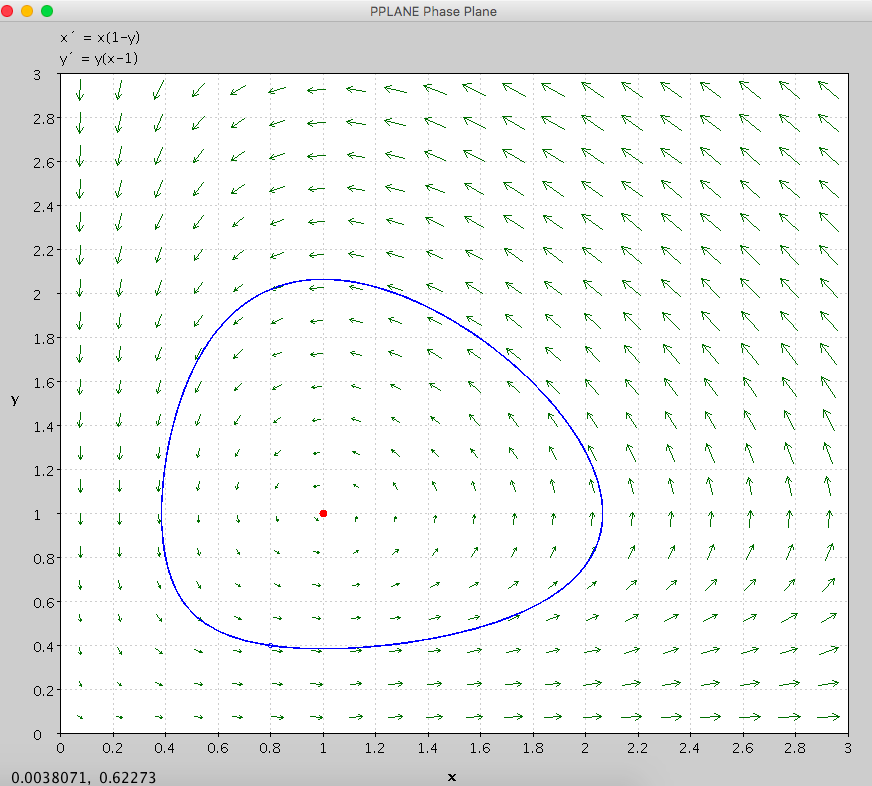
\includegraphics[scale=0.5]{img_1_y.png} 
From the graph we could see the x is never less than 0.3million(300,000) so it's not eradicated as well. And the ladybug (y axis) is greater than 2 so it will exceed 2million
\subsubsection{2}
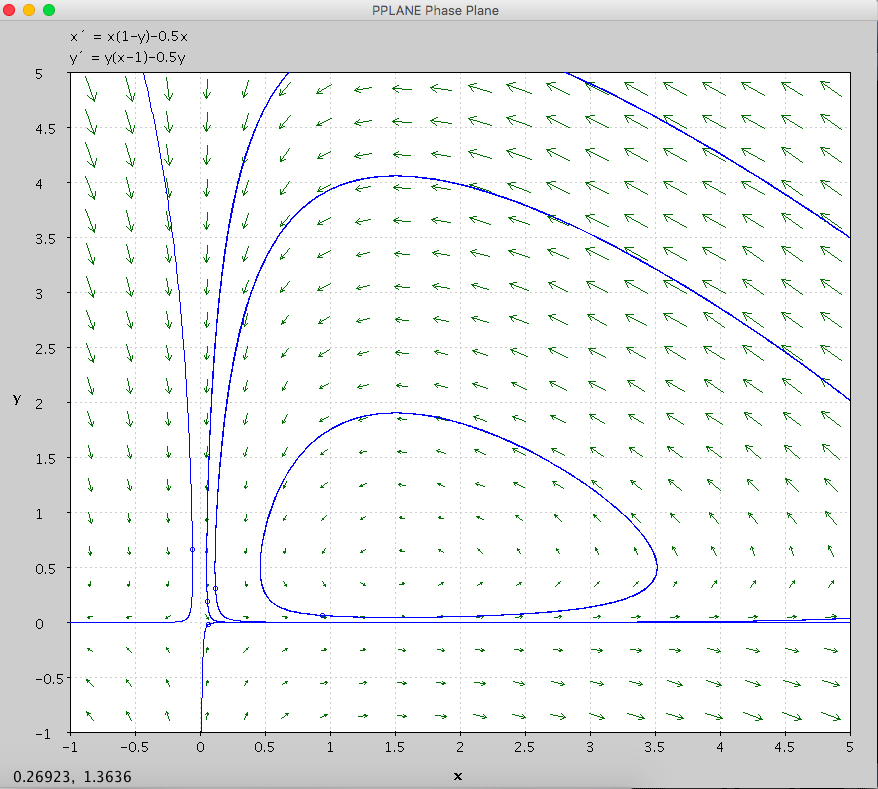
\includegraphics[scale=0.5]{img_2_05_y.png} 
From the graph we could see that the x is never becoming 0 so it won't be eradicated for s =0.5 \\
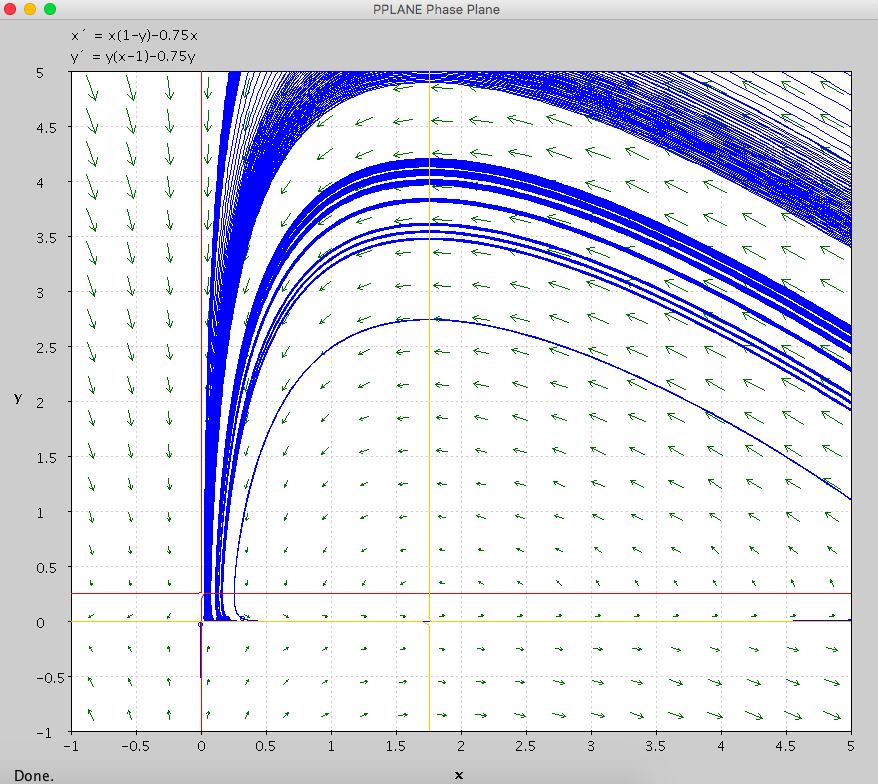
\includegraphics[scale=0.5]{img_2_075_y.png} \\
From the graph we could see that the x is never becoming 0 so it won't be eradicated. as well for s=0.75
\subsubsection{3}
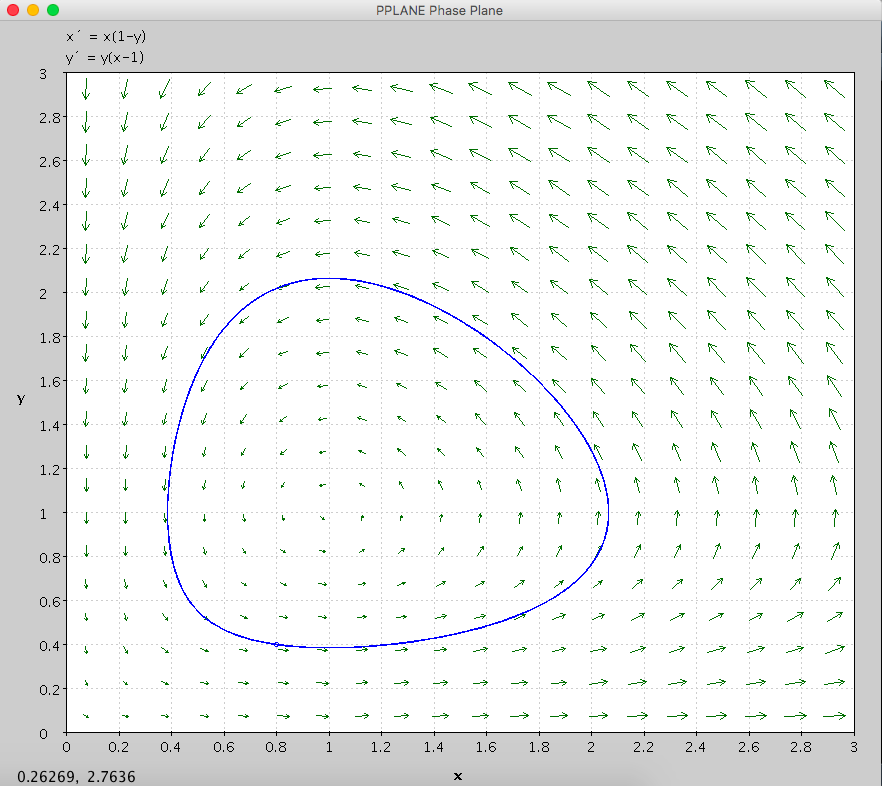
\includegraphics[scale=0.5]{img_3_0.png} \\
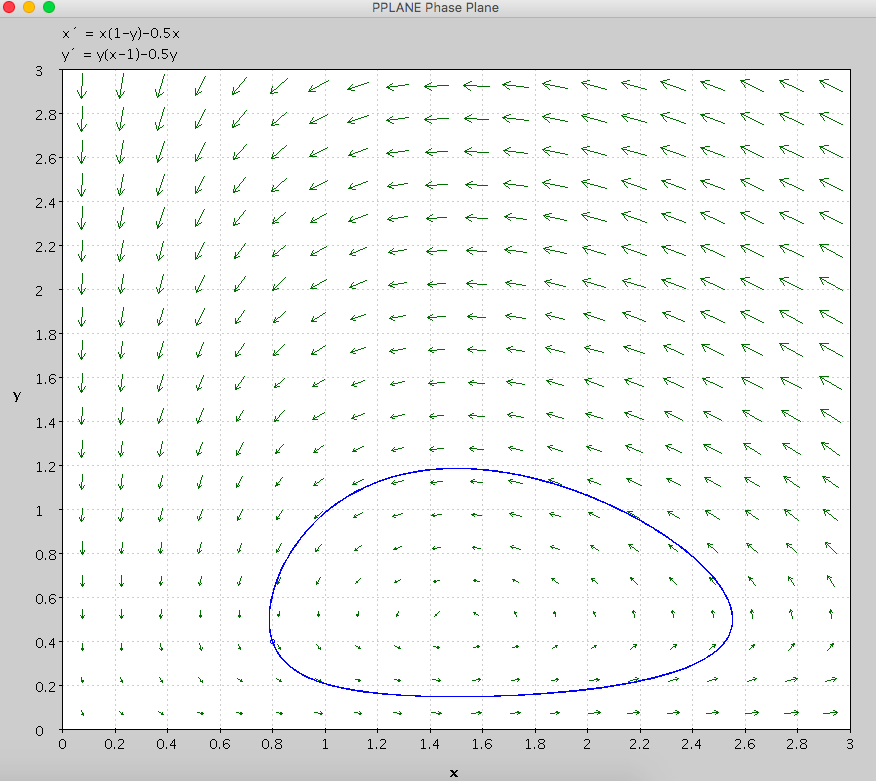
\includegraphics[scale=0.5]{img_3_05.png} \\
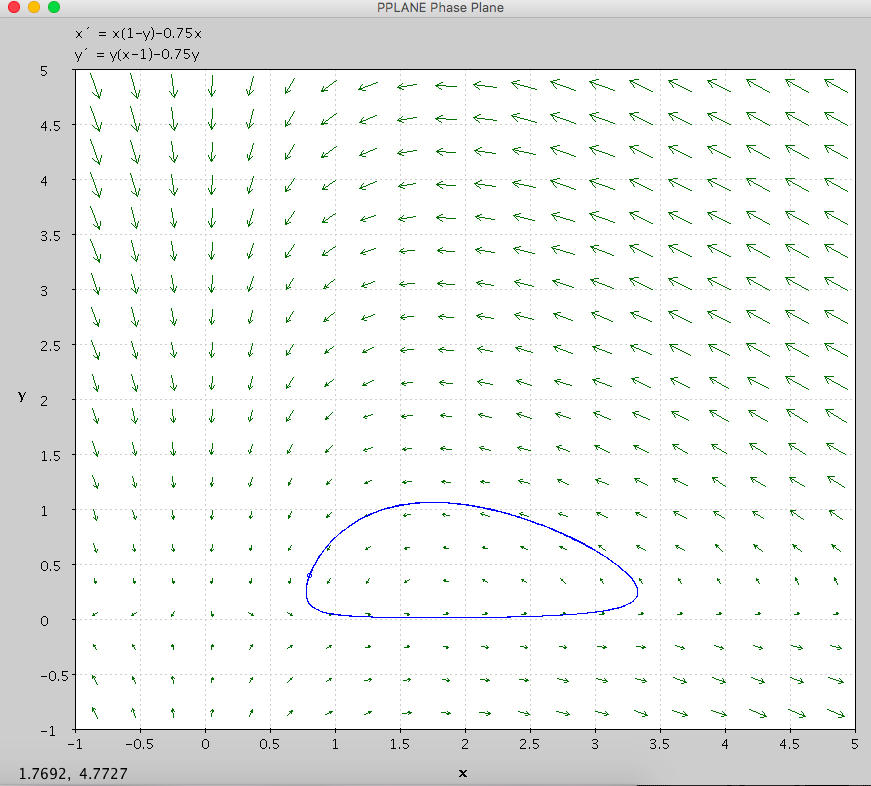
\includegraphics[scale=0.5]{img_3_075.png} \\
From the plot above we could see it would work for s=0 and s=0.5
\subsubsection{4}
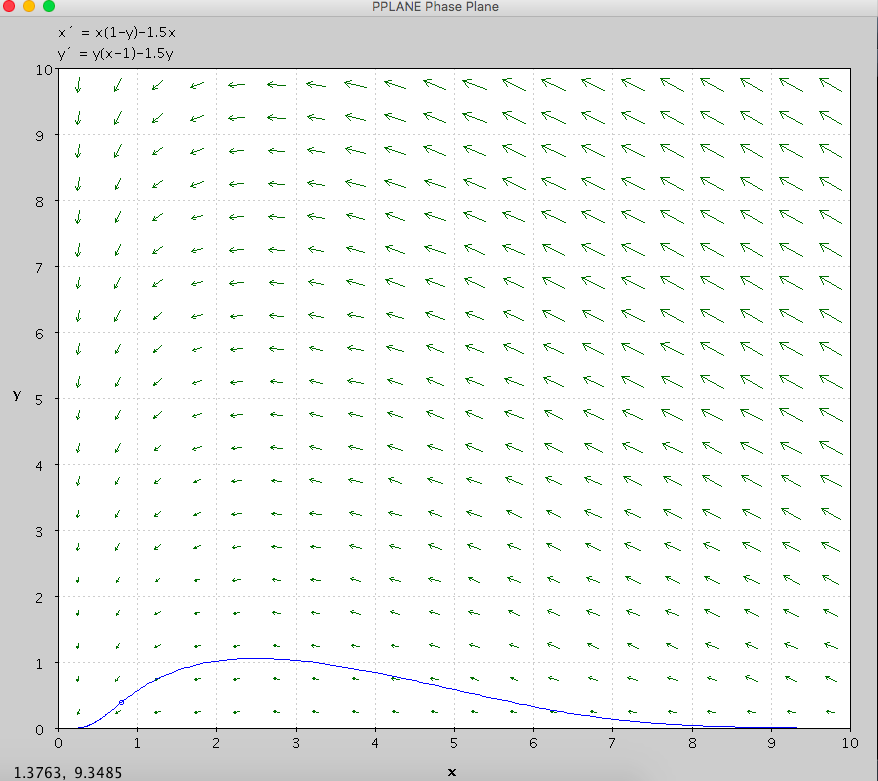
\includegraphics[scale=0.5]{img_4_0_y.png} \\
As you can see on the graph, both bugs will be eradicated

\end{homeworkProblem}



\end{document}
